\documentclass{article}
\usepackage{array}
\usepackage[a4paper, top=3cm, bottom=2.5cm, left=2.5cm, right=2.5cm]{geometry} % Ajuste de márgenes
\usepackage[spanish]{babel}
\usepackage[utf8]{inputenc}
\usepackage{tikz}
\usepackage{titling}
\usepackage{graphicx}
\usepackage{fancyhdr}
\usepackage{amsmath}
\usepackage{amssymb}
\usepackage{multicol}
\usepackage{cancel}
\usepackage{pgfplots}
\usepackage{hyperref}
\usepackage{bookmark}
\usepackage{tabularx}
\pgfplotsset{compat=1.18}
\usepackage{titlesec} % Para personalizar títulos
\usepackage{tocloft}  % Para mejorar el índice
\usepackage{setspace} % Para controlar el espaciado

\usepackage{xcolor}
\usepackage{colortbl} % Required for \rowcolor
\definecolor{azulun}{RGB}{0, 51, 102} % Define the color azulun
\usepackage{enumitem}

\definecolor{headerblue}{RGB}{50,90,140}
\definecolor{responsegray}{RGB}{80,80,80}



% Configuración de Fancyhdr para encabezados y pies de página
\pagestyle{fancy}
\fancyhf{}
\fancyhead[L]{
\includegraphics[width=2cm]{assets/logo-utp.png}}
\fancyhead[R]{\textbf{Diseño de Productos y Servicios}}

\fancyfoot[R]{\thepage} % Número de página alineado a la derecha

% Ajustes de espaciado entre párrafos y márgenes superiores
\setlength{\parskip}{1.5em}
\setlength{\parindent}{0pt}
\setlength{\headheight}{17.26935pt} % Altura del encabezado
\addtolength{\topmargin}{-2.26935pt} % Compensar el aumento de la altura del encabezado
\setlength{\textheight}{23cm}  % Ajusta el alto del texto

% Definición de comandos personalizados
\newcommand{\SubItem}[1]{
    {\setlength\itemindent{15pt} \item[-] #1}
}

% Título del documento con mejor control de espaciado
\title{
  
\includegraphics[width=5cm]{./assets/logo-utp.png} \\
  \vspace{1cm}
  \textbf{Universidad Tecnológica del Perú} \\
  \vspace{2cm}
  \textbf{Avance de Proyecto 2:\\Sistema de Reservas de Salas de Estudio.\\\textit{Sala de estudios SS}} \\
  \vspace{1cm}
  \large \textbf{Para el curso de Diseño de Productos y Servicios.} \\
  \large \textbf{Ing. Software y Sistemas.}
}
\author{
  \text{Luis Huatay Salcedo.} \\
  \text{Garcia Chumpitaz Cindel Roxell.} \\
  \text{Díaz Benítez, Fernando Raúl.} \\
  \text{Quispe Fernandez, Bryan Alexander.}
}


\begin{document}
\maketitle
\begin{center}
  Sección 44698
\end{center}
\thispagestyle{empty}
\begin{center}
  Mg. Marcos Teodoro Yerren Huima  
\end{center}
\restoregeometry

\newpage
\begin{center}
  \textbf{\Large Índice}
\end{center}
\vspace{0.5cm} % Espacio entre título y contenid
\begin{spacing}{1.15} % Espaciado personalizado para mayor legibilidad
  \noindent
  \begin{enumerate}
    \item Introducción
    \item Definición del problema
    \item Investigación de usuarios (Semana 2)
    \item Mapa de empatía
    \item Perfil de usuario, protopersona y segmentación de mercado (Semana 3)
    \item Usuario extremo (Semana 4)
    \item Lluvia de Ideas (Semana 1)
    \item Hipótesis de diseño basada en el usuario
    \item Propuesta de solución de acuerdo a la hipótesis de diseño. (Semana 5)
    \item Benchmarking y propuesta de valor (Semana 6)
    \item Storyboard
    \item Producto mínimo viable (MVP)
    \item Criterios de viabilidad o factibilidad.
  %   \begin{enumerate}
  %     \item Objetivos específicos
  %   \end{enumerate}
  %   \item Términos estadísticos
  %   \item Recolección de información
    \end{enumerate}
\end{spacing}

\newpage
\vspace*{\fill}
\section{Introducción}
La Universidad Tecnológica del Perú (UTP) es una institución educativa que ofrece una amplia gama de programas académicos y servicios a sus estudiantes. Uno de los aspectos fundamentales para el éxito académico es la disponibilidad de espacios adecuados para el estudio y la colaboración. En este contexto, el presente informe se centra en la creación de un sistema de reservas de salas de estudio, diseñado específicamente para satisfacer las necesidades de los estudiantes y mejorar su experiencia educativa.

El sistema de reservas de salas de estudio tiene como objetivo facilitar la gestión y el uso eficiente de los espacios de estudio disponibles en la UTP. A través de este sistema, los estudiantes podrán reservar salas de estudio de manera rápida y sencilla, asegurando así un entorno propicio para el aprendizaje y la colaboración.
\vspace*{\fill}

\newpage

\section{Definición del problema}

Muchos estudiantes tienen dificultades para reservar salas de estudio en la biblioteca 
debido a la falta de un sistema digital eficiente. Esto genera desorganización, pérdida de tiempo y conflictos por el uso de espacios.

La UTP cuenta con una biblioteca que ofrece diversas salas de estudio, pero la gestión de reservas que se realiza por su aplicación se hace de manera que una sala está completamente ocupada por el tiempo que se reserva y no por el tiempo que se ocupa, lo que puede llevar a confusiones y malentendidos entre los estudiantes. Además, la falta de un sistema centralizado dificulta la planificación y el uso óptimo de estos espacios.

La situación actual presenta varios problemas, entre ellos:
\begin{itemize}
    \item Falta de un sistema digital eficiente para la gestión de reservas.
    \item Desorganización en la utilización de los espacios de estudio.
    \item Conflictos entre estudiantes por el uso de las salas.
    \item Dificultad para encontrar y reservar salas de estudio disponibles.
    \item Pérdida de tiempo al buscar espacios adecuados para estudiar.
    \item Falta de información sobre la disponibilidad de salas en tiempo real.
\end{itemize}

\subsection{¿Qué problema o necesidad busca solucionar su proyecto?}

El proyecto busca implementar una plataforma web o app que permita a los estudiantes 
reservar salas de forma rápida, ordenada y sobre todo, que estas se mantengan disponibles a penas se desocupan. Esto no solo mejorará la experiencia de los estudiantes, sino que también optimizará el uso de los espacios de estudio en la UTP.

\subsection{¿Nos es posible resolver el problema?}

La implementación de un sistema de reservas de salas de estudio es factible y puede llevarse a cabo mediante el desarrollo de una plataforma web o aplicación móvil. Esta solución permitirá a los estudiantes gestionar sus reservas de manera eficiente, evitando conflictos y mejorando la organización en el uso de los espacios de estudio.
Además, la tecnología actual permite la integración de funciones como notificaciones en tiempo real, gestión de horarios y disponibilidad de salas, lo que facilitará aún más el proceso de reserva.

\newpage

\section{Investigación de usuarios}

La investigación de usuarios es un proceso fundamental para comprender las necesidades y expectativas de los estudiantes en relación con el sistema de reservas de salas de estudio. A través de encuestas y entrevistas, se recopilará información valiosa que guiará el diseño y desarrollo del sistema.
\vspace{-0.5cm}
\subsection{Preguntas de entrevista}

Las preguntas de entrevista se caracterizan por ser abiertas y permitir a los usuarios expresar sus opiniones y experiencias de manera detallada. A continuación, se presentan algunas preguntas que se utilizarán en las entrevistas:

\begin{enumerate}
  \item ¿Cuánto tiempo sueles usar una sala de estudio por sesión?
  \item ¿Qué dificultades tienes al acceder a las salas de estudio? ¿Por qué?
  \item ¿Qué funciones te parecerían más útiles en un sistema de reservas para las salas de estudio?
  \item ¿Qué tan fácil te resulta usar el sistema de reservas y qué cambiarías para mejorarlo?
  \item ¿Crees que un sistema de reservas eficiente influye en tus actividades académicas? ¿Por qué?
\end{enumerate}

\subsection{Preguntas de encuesta}

Esta por otro lado, se caracteriza por ser cerrada y permite obtener datos cuantitativos. Estas preguntas están construidas bajo escala Likert, donde los encuestados pueden seleccionar una opción que mejor represente su opinión, además, se incluyen preguntas de respuesta dicotómica (Sí/No) y de opción múltiple. A continuación, se presentan algunas preguntas que se utilizarán en la encuesta:

\begin{multicols}{2}
  \begin{enumerate}
    \item ¿Tu universidad cuenta con un sistema de reservas para las salas de estudio? 
    \begin{itemize}[label=$\square$]
      \item a) Sí
      \item b) No
    \end{itemize}
  
    \item ¿Con qué frecuencia utilizas las salas de estudio? (Escala Likert)
    \begin{itemize}[label=$\square$]
      \item 1) Nunca
      \item 2) Rara vez
      \item 3) Ocasionalmente
      \item 4) Frecuentemente
      \item 5) Siempre
    \end{itemize}
  
    \item ¿El horario actual de las salas de estudio satisface tus necesidades? 
    \begin{itemize}[label=$\square$]
      \item a) Sí
      \item b) No
    \end{itemize}
  
    \item ¿Qué tan satisfecho/a estás con la disponibilidad de las salas? (Escala Likert)
    \begin{itemize}[label=$\square$]
      \item 1) Muy insatisfecho/a
      \item 2) Insatisfecho/a
      \item 3) Neutral
      \item 4) Satisfecho/a
      \item 5) Muy satisfecho/a
    \end{itemize}
  
    \item ¿Has tenido problemas para encontrar salas disponibles? 
    \begin{itemize}[label=$\square$]
      \item a) Sí
      \item b) No
    \end{itemize}
  
    \item ¿Qué tan útil consideras que sería una aplicación de reservas? (Escala Likert)
    \begin{itemize}[label=$\square$]
      \item 1) Nada útil
      \item 2) Poco útil
      \item 3) Neutral
      \item 4) Útil
      \item 5) Muy útil
    \end{itemize}
  \end{enumerate}  
\end{multicols}

\newpage
\section{Mapa de empatía}

Esta sección pretende resumir la información obtenida de los usuarios a través de las entrevistas y encuestas. El mapa de empatía es una herramienta visual que ayuda a comprender mejor a los usuarios y sus necesidades. A continuación, se presenta un ejemplo de un mapa de empatía para el sistema de reservas de salas de estudio:

\begin{center}
  \begin{tabular}{|>{\centering\arraybackslash}m{3cm}|>{\centering\arraybackslash}p{11cm}|}
    \hline
    \textbf{¿Qué piensa y siente?} & 
    \begin{itemize}[leftmargin=*, label={--}]
      \item Deseo de la implementación de un sistema de reservas de sala de estudio.
      \item Requiere estudiar en un ambiente tranquilo, sin bulla ni distracciones.
      \item No estar haciendo cola para pedir una reserva de manera presencial.
    \end{itemize} \\ \hline
    \textbf{¿Qué ve?} & 
    \begin{itemize}[leftmargin=*, label={--}]
      \item Sistemas que tienen poco diseño orientado al usuario.
      \item Dificultades para guiarse dentro de la plataforma.
      \item Solicitud de los estudiantes por mejoras en los sistemas de reserva.
    \end{itemize} \\ \hline
    \textbf{¿Qué escucha?} & 
    \begin{itemize}[leftmargin=*, label={--}]
      \item Comentarios de otros estudiantes con problemas similares.
      \item Sugerencias para añadir más funciones al sistema.
      \item Preferencias de sesiones de estudio grupales frente a las individuales.
    \end{itemize} \\ \hline
    \textbf{¿Qué dice y hace?} & 
    \begin{itemize}[leftmargin=*, label={--}]
      \item De manera general, el uso de las salas es ocasionalmente.
      \item Solicita mejoras en la interfaz del sistema.
      \item Preferencias por las salas de estudio en el turno de mañana.
    \end{itemize} \\ \hline
    \textbf{¿Cuáles son sus esfuerzos?} & 
    \begin{itemize}[leftmargin=*, label={--}]
      \item Dificultades para conseguir una sala de estudio por motivo de ocupación.
      \item Demora del sistema en conseguir salas de estudio.
      \item Problemas con la experiencia del usuario.
    \end{itemize} \\ \hline
    \textbf{¿Qué resultados espera?} & 
    \begin{itemize}[leftmargin=*, label={--}]
      \item Reservas garantizadas en todos los horarios.
      \item Mejoras en el sistema como notificaciones cuando el tiempo de uso de la sala culmine.
      \item Mejor gestión del uso de las salas.
    \end{itemize} \\ \hline
  \end{tabular}
\end{center}

\newpage

\section{Perfil de usuario, protopersona y segmentación de mercado}

El perfil de usuario es una representación ficticia de un usuario típico del sistema de reservas de salas de estudio. A continuación, se presenta un perfil de usuario que resume las características y necesidades de los estudiantes, además de una protopersona que representa a un usuario específico:

\subsection{Perfil de Usuario}

\textbf{Sistema de Reservas de Salas en la Biblioteca:} Estudio universitario \\
\textbf{Edad:} 18 a 26 años \\
\textbf{Profesión:} Sin especificar \\
\textbf{Necesidad principal:} El estudiante requiere un espacio de estudio que garantice la concentración y el aprendizaje, libre de interrupciones externas, y que además le permita reservar dicha sala de manera remota sin necesidad de acudir a las oficinas del Servicio Estudiantil.

\subsection{Proto-persona}

\textbf{Nombre:} Camilo Soza \\
\textbf{Edad:} 20 años \\
\textbf{Carrera:} Derecho \\
\textbf{Motivaciones:} Le gusta la investigación de temas referentes al derecho penal. \\
\textbf{Frustraciones:} El estudiante se siente frustrado por la falta de un espacio de estudio adecuado dentro de la universidad para realizar sus actividades, y le resulta incómodo esperar largos periodos en la cola del Servicio Estudiantil, donde otros estudiantes realizan consultas diversas.

\subsection{Segmentación de mercado}
\textbf{Segmento de mercado:} Estudiantes universitarios de la UTP \\
\textbf{Características demográficas:} Estudiantes de 18 a 26 años, de diversas carreras académicas. \\
\textbf{Características psicográficas:} Estudiantes que valoran la eficiencia y la comodidad en el acceso a los recursos de estudio. \\
\textbf{Comportamiento:} Estudiantes que utilizan regularmente las salas de estudio y buscan una solución digital para gestionar sus reservas. \\
\textbf{Necesidades:} Acceso rápido y fácil a las salas de estudio, información en tiempo real sobre la disponibilidad de espacios, y una experiencia de usuario intuitiva.

\newpage

\section{Usuario extremo}

El usuario extremo es una representación de un usuario que tiene necesidades y expectativas muy específicas en relación con el sistema de reservas de salas de estudio. A continuación, se presenta un ejemplo de un usuario extremo:

\textbf{Nombre:} María López \\
\textbf{Edad:} 57 años \\
\textbf{Carrera:} Derecho \\
\textbf{Motivaciones:} María es una estudiante de posgrado que trabaja a tiempo completo y tiene un horario muy ajustado. Necesita un sistema de reservas que le permita gestionar su tiempo de manera eficiente y asegurarse de que siempre haya una sala disponible cuando la necesite. 

\subsection{Preguntas y respuestas del usuario extremo:}

\begin{enumerate}

  \item \textbf{¿Cuánto tiempo sueles usar una sala de estudio por sesión? }
    
    \hspace{1cm}\textit{Generalmente, utilizo las salas de estudio durante 2 horas, pero a veces necesito quedarme más tiempo para terminar mis tareas.}

  \item \textbf{¿Qué dificultades tienes al acceder a las salas de estudio? ¿Por qué?}  
    
    \hspace{1cm}\textit{A menudo encuentro que las salas están ocupadas o que no hay disponibilidad en el horario que necesito. Además, el sistema actual es confuso y no me permite hacer reservas fácilmente.}

  \item \textbf{¿Qué funciones te parecerían más útiles en un sistema de reservas para las salas de estudio?}  
    
    \hspace{1cm}\textit{Me gustaría poder ver la disponibilidad de las salas en tiempo real y recibir notificaciones cuando haya una sala libre. También sería útil poder reservar varias horas a la vez.}

  \item \textbf{¿Qué tan fácil te resulta usar el sistema de reservas y qué cambiarías para mejorarlo?}  
    
    \hspace{1cm}\textit{El sistema actual es complicado y no es intuitivo. Cambiaría la interfaz para que sea más amigable y fácil de usar. También me gustaría tener una opción de ayuda o tutorial.}

  \item \textbf{¿Crees que un sistema de reservas eficiente influye en tus actividades académicas? ¿Por qué?}  
    
    \hspace{1cm}\textit{Definitivamente. Un sistema de reservas eficiente me permitiría planificar mejor mi tiempo y asegurarme de que tengo un lugar para estudiar cuando lo necesito.}

  \end{enumerate}

  \subsection{Descripción de los hallazgos}

  \begin{itemize}
    \item María tiene un horario muy ajustado y necesita un sistema de reservas que le permita gestionar su tiempo de manera eficiente.
    \item La disponibilidad de las salas es un problema recurrente para ella, lo que afecta su capacidad para estudiar.
    \item La interfaz del sistema actual es confusa y no le permite hacer reservas fácilmente.
    \item María valora la posibilidad de recibir notificaciones sobre la disponibilidad de salas y la opción de reservar varias horas a la vez.
    \item Un sistema de reservas eficiente influiría positivamente en sus actividades académicas, permitiéndole planificar mejor su tiempo y asegurarse de que tiene un lugar para estudiar.
    \item María es un usuario extremo que representa a aquellos estudiantes con horarios ajustados y necesidades específicas en relación con el sistema de reservas de salas de estudio.
    \item La implementación de un sistema de reservas eficiente y fácil de usar podría mejorar significativamente la experiencia de María y otros estudiantes en situaciones similares.
  \end{itemize}

  \section{Lluvia de ideas}
  
  Llamada también como \textit{brainstorming}, es una técnica de generación de ideas que busca fomentar la creatividad y la colaboración entre los miembros del equipo. A continuación, se presentan algunas ideas generadas durante la lluvia de ideas para el sistema de reservas de salas de estudio:

  \begin{table}[h]
    \centering
    
    \label{tab:ideas}
    \begin{tabular}{|>{\color{azulun}\bfseries}l|p{10cm}|}
    \hline
    \rowcolor{azulun!20}
    \textcolor{white}{\textbf{\#}} & \textcolor{white}{\textbf{Idea}} \\
    \hline
    1 & \textbf{Aplicación móvil integrada} \\ 
    & Desarrollo de una app multiplataforma (iOS/Android) con autenticación SSO mediante credenciales universitarias, que muestre en tiempo real la disponibilidad de salas. \\
    \hline
    2 & \textbf{Sistema de puntuación y recompensas} \\ 
    & Implementar un sistema que otorgue puntos por el uso responsable (dejar limpio, respetar horarios) canjeables por beneficios académicos. \\
    \hline
    3 & \textbf{Integración con calendario académico} \\ 
    & Sincronización automática con el calendario de la universidad para priorizar reservas durante periodos de exámenes o entregas de proyectos. \\
    \hline
    4 & \textbf{Salas temáticas inteligentes} \\ 
    & Habilitar salas con equipamiento específico (proyectores, pizarras digitales) y sistema de detección automática de ocupación mediante sensores IoT. \\
    \hline
    5 & \textbf{Sistema de préstamo de llaves digital} \\ 
    & Uso de tecnología NFC/Bluetooth para desbloquear salas mediante el smartphone, eliminando llaves físicas y controles manuales. \\
    \hline
    6 & \textbf{Analítica predictiva} \\ 
    & Módulo de inteligencia artificial que anticipe la demanda por facultad/horario y sugiera horarios alternativos con menor congestión. \\
    \hline
    
    \end{tabular}
    \caption{Ideas de brainstorming para sistema de reservas de salas}
    \end{table}

    \newpage

  \section{Hipótesis de diseño basada en el usuario.}

  \textbf{Hipótesis de diseño:} Si implementamos un sistema de reservas de salas de estudio que permita a los estudiantes gestionar sus reservas de manera eficiente y recibir notificaciones en tiempo real, entonces mejoraremos la experiencia de los estudiantes y optimizaremos el uso de los espacios de estudio en la UTP.

  Sin duda, el valor que se propone radica en cambiar el paradigma de reservas de la típica reserva por cantidad de tiempo que resulta en la ocupación de una sala, a un sistema que permita reservar por tiempo de uso. Esto no solo mejorará la experiencia de los estudiantes, sino que también optimizará el uso de los espacios de estudio en la UTP.

  \textbf{Justificación:} Este sistema de reservas permitirá a los estudiantes acceder a las salas de estudio de manera más eficiente, evitando conflictos y mejorando la organización en el uso de estos espacios. Además, la implementación de un sistema digital facilitará la gestión y el acceso a la información sobre la disponibilidad de salas, lo que contribuirá a una experiencia de usuario más satisfactoria.

  La justificación de esta hipótesis se basa en la necesidad de los estudiantes de contar con un sistema que les permita gestionar sus reservas de manera eficiente y optimizar el uso de los espacios de estudio. La implementación de un sistema digital que permita a los estudiantes reservar salas de estudio de manera rápida y sencilla contribuirá a mejorar su experiencia académica y facilitará el acceso a los recursos necesarios para su aprendizaje.

  \section{Propuesta de solución de acuerdo a la hipótesis de diseño.}

  La propuesta de solución consiste en el desarrollo de un sistema de reservas de salas de estudio que permita a los estudiantes gestionar sus reservas de manera eficiente y recibir notificaciones en tiempo real. Este sistema estará disponible a través de una plataforma web y una aplicación móvil, lo que facilitará su acceso y uso por parte de los estudiantes.
  \subsection{Características del sistema:}
  \begin{itemize}
    \item Interfaz amigable y fácil de usar.
    \item Visualización en tiempo real de la disponibilidad de salas.
    \item Opción de reservar varias horas a la vez.
    \item Notificaciones automáticas sobre la disponibilidad de salas.
    \item Integración con el calendario académico de la UTP.
    \item Sistema de puntuación y recompensas por el uso responsable de las salas.
    \item Salas temáticas inteligentes con equipamiento específico.
    \item Sistema de préstamo de llaves digital mediante tecnología NFC/Bluetooth.
    \item Analítica predictiva para anticipar la demanda por facultad/horario.
    \item Sistema de gestión de reservas que permita a los estudiantes cancelar o modificar sus reservas de manera sencilla.
    \item Sistema de soporte técnico y atención al usuario para resolver dudas y problemas relacionados con el uso del sistema.
    \end{itemize}
  \subsection{Beneficios esperados:}
  \begin{itemize}
    \item Mejora en la experiencia de los estudiantes al acceder a las salas de estudio.
    \item Optimización del uso de los espacios de estudio en la UTP.
    \item Reducción de conflictos y desorganización en la gestión de reservas.
    \item Facilitar la planificación y el uso eficiente de los recursos disponibles.
    \item Aumento en la satisfacción de los estudiantes con respecto a los servicios ofrecidos por la universidad.
    \end{itemize}

    \subsection{Solución bajo el punto de vista del usuario: \textbf{Job To Be Done}}

    \textbf{¿Qué trabajo necesita hacer el usuario?} El usuario necesita gestionar sus reservas de salas de estudio de manera eficiente y optimizar su tiempo de estudio.

    En ese sentido, se hace uso del concepto de \textbf{Job To Be Done} (JTBD), que se refiere a la tarea o trabajo que el usuario necesita realizar. En este caso, el trabajo que el usuario necesita hacer es gestionar sus reservas de salas de estudio de manera eficiente y optimizar su tiempo de estudio. Esto implica que el sistema debe permitir al usuario realizar reservas de manera rápida y sencilla, así como recibir notificaciones sobre la disponibilidad de salas y gestionar sus reservas de manera flexible.

    \section{Benchmarking y propuesta de valor}

    El benchmarking es una técnica que consiste en comparar el rendimiento y las características de un producto o servicio con los de la competencia. En este caso, se realizará un análisis comparativo de sistemas de reservas de salas de estudio existentes en otras universidades y plataformas similares.

    \subsection{Análisis de la competencia}
    \begin{itemize}
      \item \textbf{Sistema de reservas en otras universidades:} Muchas universidades cuentan con sistemas de reservas de salas de estudio, pero la mayoría de ellos son limitados en cuanto a funcionalidades y no ofrecen una experiencia de usuario satisfactoria.
      
      \item \textbf{El Coworking:} Esta plataforma permite a los usuarios reservar espacios de trabajo y salas de estudio, pero su enfoque está más orientado a espacios de coworking que a salas de estudio universitarias.
      \end{itemize}

      Como se puede observar, la mayoría de los sistemas de reservas existentes presentan limitaciones en cuanto a funcionalidades y experiencia de usuario. Esto representa una oportunidad para desarrollar un sistema de reservas de salas de estudio que ofrezca una experiencia de usuario superior y funcionalidades avanzadas.

      \subsection{Cuadro comparativo de productos}

      Competencia: \textbf{Starbucks} - \textbf{Bembos}

\begin{table}[ht]
  \centering
  \scriptsize
  % Ajuste automático de ancho con tabularx
  \begin{tabularx}{\textwidth}{|>{\raggedright\arraybackslash}X|>{\raggedright\arraybackslash}X|>{\raggedright\arraybackslash}X|>{\raggedright\arraybackslash}X|>{\raggedright\arraybackslash}X|>{\raggedright\arraybackslash}X|}
  \hline
  \textbf{Producto} & \textbf{Público objetivo} & \textbf{Principales funciones} & \textbf{Fortalezas} & \textbf{Debilidades} & \textbf{Valor diferenciador} \\
  \hline
  Sala de estudios & Estudiantes  & Reserva inteligente por disponibilidad  & Solicitud de servicios externos; gratuito  & Salas limitadas; aire acondicionado compartido; espacio reducido  & Gratis frente a la competencia  \\
  \hline
  Starbucks & Público general  & Venta de productos y servicio de cafetería  & Atención rápida; ambiente atractivo  & Sin pizarras; sin computadoras; internet lento  & Experiencia cuidada y consistente  \\
  \hline
  Bembos & Público general  & Comida rápida; opción de almuerzo  & Precios accesibles; menú variado  & Ambiente ruidoso; no propicio para el estudio  & Espacios recreativos para niños  \\
  \hline
  \end{tabularx}
  \caption{Comparación de productos y su propuesta de valor ajustada}
  \label{tab:comparacion-productos}
  \end{table}

      \subsection{Propuesta de valor}

      La propuesta de valor del sistema de reservas de salas de estudio se basa en ofrecer una solución integral que permita a los estudiantes gestionar sus reservas de manera eficiente y optimizar su tiempo de estudio. Esto incluye una interfaz amigable, notificaciones en tiempo real, integración con el calendario académico y un sistema de puntuación y recompensas por el uso responsable de las salas.

      \begin{description}[leftmargin=2cm,style=nextline]
        \item[Para] \textbf{estudiantes}
        \item[que necesitan] \textbf{salas / espacio de estudios}
        \item[nuestra solución es] \textbf{sistema de reservas}
        \item[que ofrece] \textbf{reservar salas de estudio}
        \item[a diferencia de] \textbf{mayor cantidad de servicios}
        \item[porque] \textbf{enfocado a estudiantes}
      \end{description}

      \newpage
      
      \noindent\textbf{Producto Final:}
      
      Nuestro producto final va dirigido a estudiantes universitarios que necesitan acceder y reservar espacios de estudio. Nuestra solución es un sistema de reservas en línea que ofrece confirmación instantánea y gestión de disponibilidad en tiempo real, a diferencia de las plataformas genéricas con múltiples servicios dispersos, porque está diseñado específicamente para optimizar la experiencia de estudio.

      Así mismo se propone el modelo de Lean Canvas, que es una herramienta visual que permite resumir y validar la propuesta de valor del sistema de reservas de salas de estudio. A continuación, se presenta un ejemplo de un Lean Canvas para el sistema:

      \begin{figure}[ht]
        \centering
        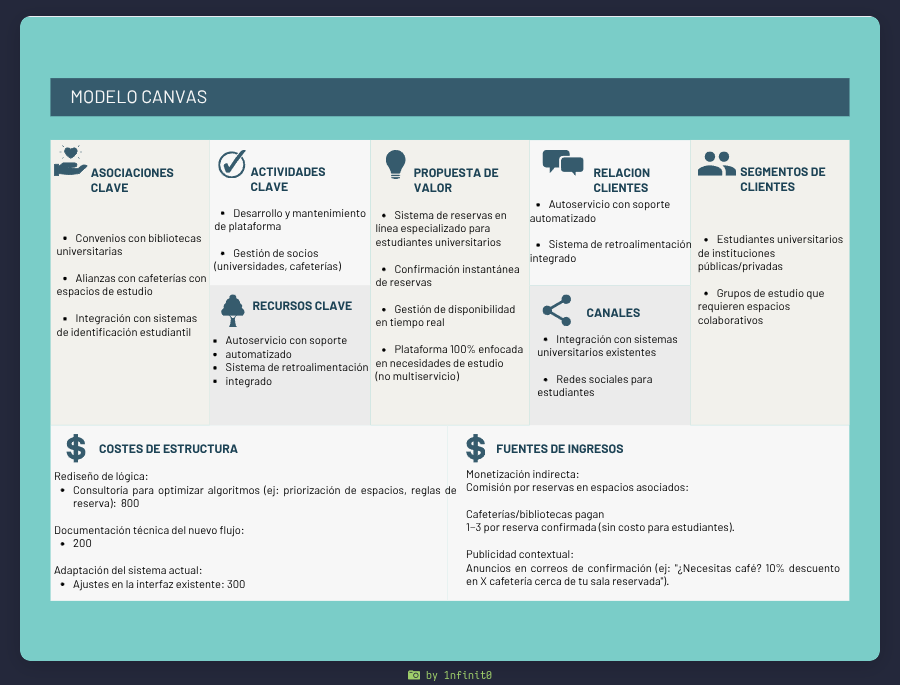
\includegraphics[width=0.9\textwidth]{assets/lean.png}
        \caption{Modelo de Lean Canvas}
        \label{fig:example-image}
      \end{figure}

      Como se puede observar, el Lean Canvas resume los aspectos clave del sistema de reservas de salas de estudio, incluyendo la propuesta de valor, los segmentos de clientes, los canales de distribución y las fuentes de ingresos. Esta herramienta es útil para validar la propuesta de valor y asegurarse de que el sistema satisfaga las necesidades de los estudiantes.


      \newpage

      \section{Storyboard}

      El storyboard es una herramienta visual que permite representar de manera gráfica el flujo de interacción del usuario con el sistema de reservas de salas de estudio. A continuación, se presenta un ejemplo de un storyboard que ilustra el proceso de reserva de una sala de estudio:

      \begin{figure}[ht]
        \centering
        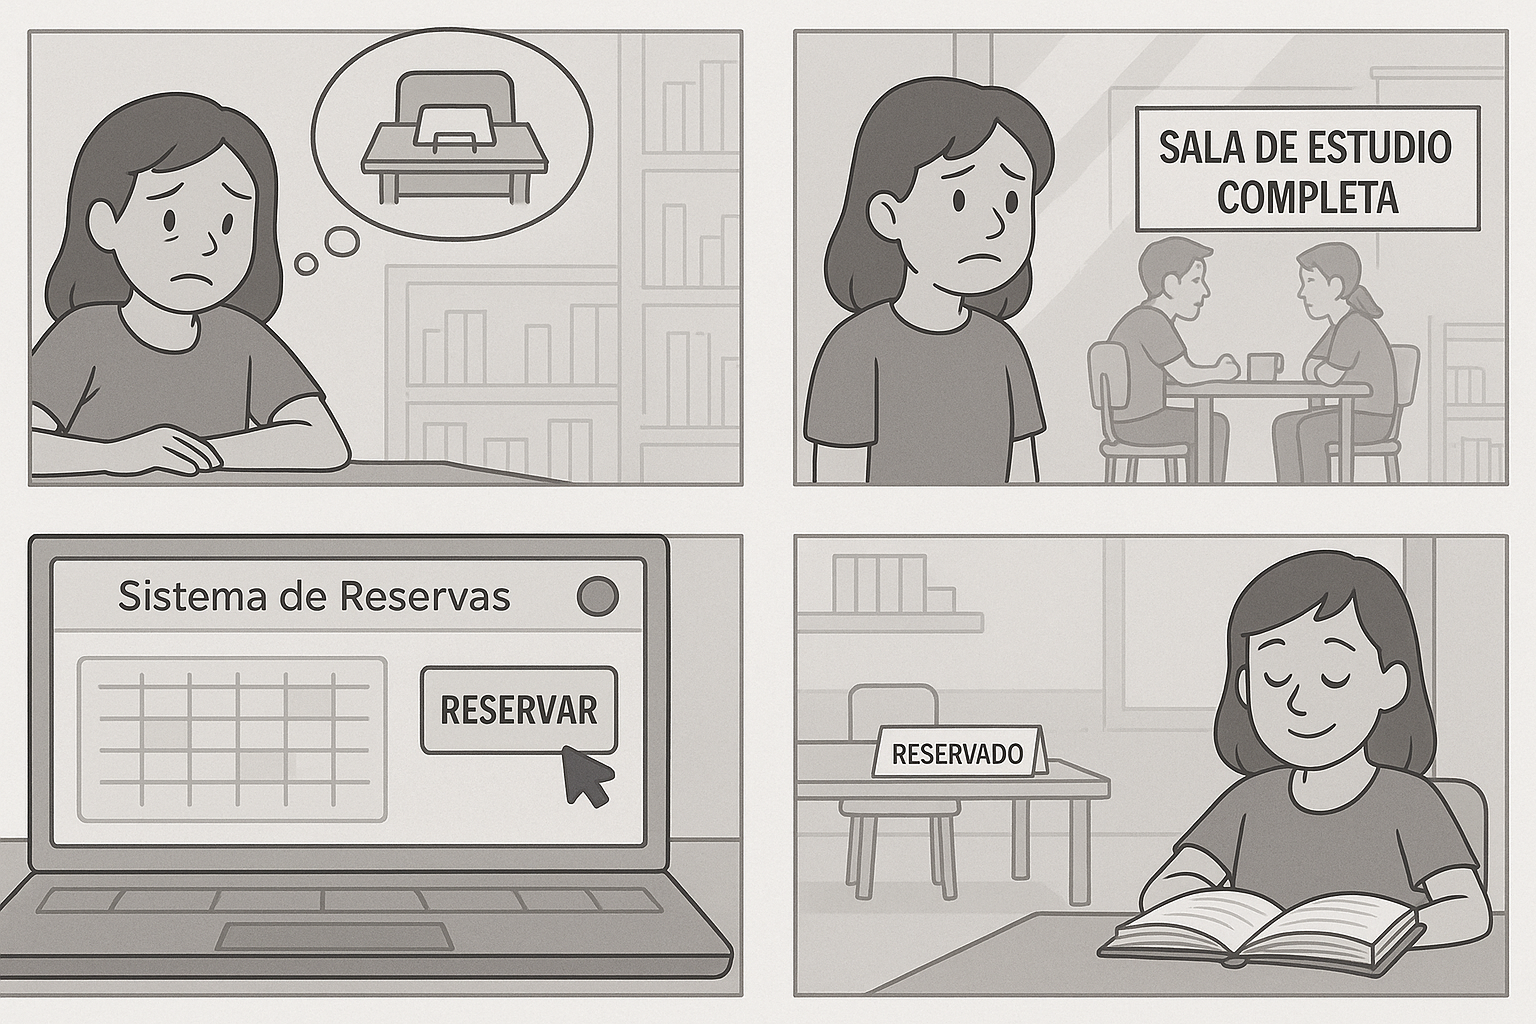
\includegraphics[width=0.9\textwidth]{assets/storyboard.png}
        \caption{Storyboard del sistema de reservas de salas
        de estudio}
        \label{fig:Storyboard}
      \end{figure}
  
      El storyboard muestra los pasos que sigue el usuario para reservar una sala de estudio, desde la selección de la sala hasta la confirmación de la reserva. Esta herramienta es útil para visualizar el flujo de interacción del usuario y asegurarse de que el sistema sea intuitivo y fácil de usar.

      Así mismo, las expresiones del usuario en cada paso del storyboard reflejan sus emociones y expectativas durante el proceso de reserva. Esto ayuda a identificar posibles puntos de fricción y áreas de mejora en la experiencia del usuario.
      \newpage

      \section{Desglose inicial del MVP}

      El Producto Mínimo Viable (MVP) es una versión simplificada del sistema de reservas de salas de estudio que incluye las funcionalidades esenciales para validar la propuesta de valor y obtener retroalimentación de los usuarios. A continuación, se presenta un desglose inicial del MVP:

      \begin{itemize}
        \item Interfaz de usuario amigable y fácil de usar.
        \item Visualización en tiempo real de la disponibilidad de salas.
        \item Opción de reservar una sala por un periodo específico.
        \item Notificaciones automáticas sobre la disponibilidad de salas.
        \item Sistema de gestión de reservas que permita a los estudiantes cancelar o modificar sus reservas.
        \item Sistema de soporte técnico y atención al usuario para resolver dudas y problemas relacionados con el uso del sistema.
        \item Sistema de autenticación mediante credenciales universitarias.
      \end{itemize}

      Así mismo, se muestra acontinuación el prototipo visual de la interfaz del sistema de reservas de salas de estudio, que ilustra cómo se verá el MVP:
      \begin{figure}[ht]
        \centering
        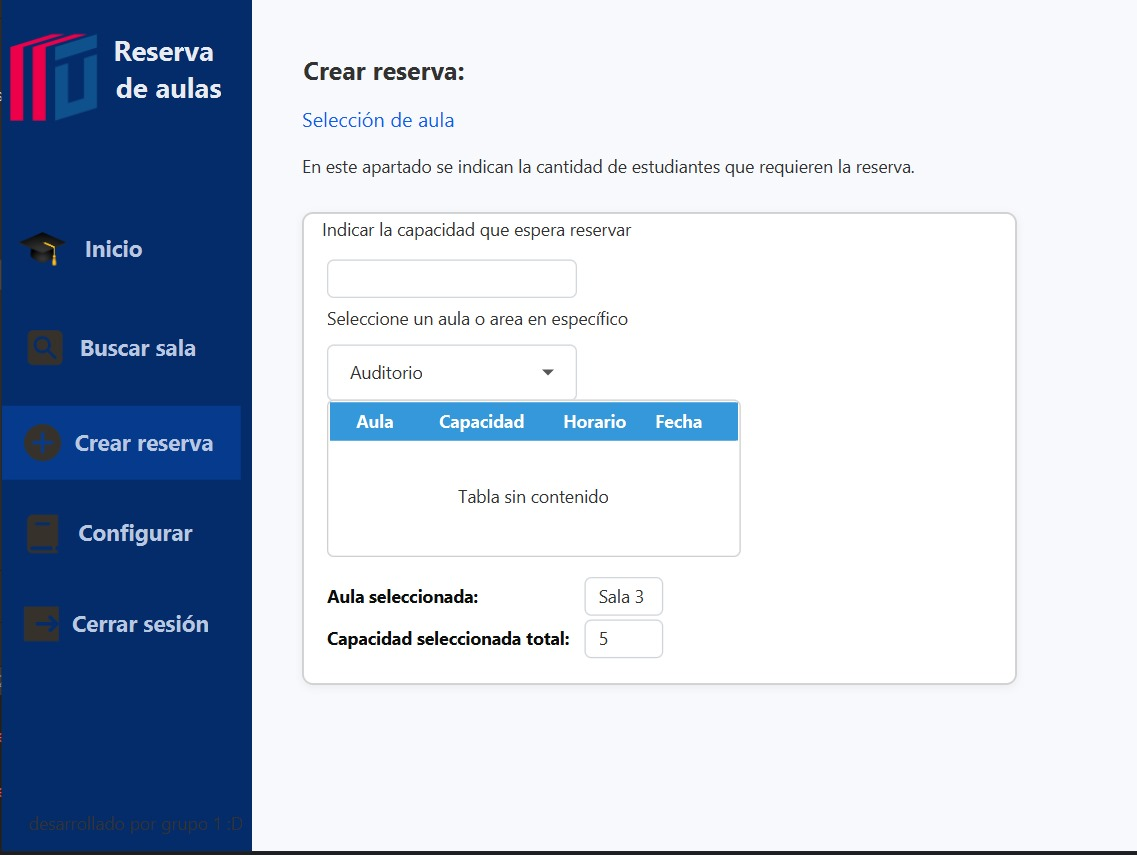
\includegraphics[width=0.9\textwidth]{assets/proto.jpeg}
        \caption{Prototipo visual del sistema de reservas de salas de estudio}
        \label{fig:prototipo}
      \end{figure}
      \newpage

      \section{Criterios de viabilidad o factibilidad}

      \subsection{Viabilidad técnica}

      La viabilidad técnica del sistema de reservas de salas de estudio se basa en la disponibilidad de tecnologías y herramientas que permiten desarrollar una plataforma web y una aplicación móvil. Además, la integración con sistemas existentes en la UTP facilitará la implementación del sistema.
      \subsection{Viabilidad económica}
      La viabilidad económica del sistema de reservas de salas de estudio se basa en la estimación de costos y beneficios asociados con la implementación del sistema. Se espera que el sistema genere ahorros en la gestión de reservas y mejore la satisfacción de los estudiantes, lo que a su vez puede aumentar la retención y el rendimiento académico.
      \subsection{Viabilidad operativa}
      La viabilidad operativa del sistema de reservas de salas de estudio se basa en la capacidad del equipo de desarrollo para implementar y mantener el sistema. Además, se espera que el sistema sea fácil de usar y que los estudiantes puedan adaptarse rápidamente a la nueva plataforma.
      \subsection{Viabilidad legal}
      La viabilidad legal del sistema de reservas de salas de estudio se basa en el cumplimiento de las normativas y regulaciones relacionadas con la protección de datos y la privacidad de los usuarios. Se espera que el sistema cumpla con las leyes y regulaciones aplicables en materia de protección de datos personales y privacidad.
      \subsection{Viabilidad temporal}
      La viabilidad temporal del sistema de reservas de salas de estudio se basa en la estimación del tiempo necesario para desarrollar e implementar el sistema. Se espera que el desarrollo del sistema se complete en un plazo razonable, lo que permitirá su implementación antes del inicio del próximo semestre académico.
      \subsection{Viabilidad social}
      La viabilidad social del sistema de reservas de salas de estudio se basa en la aceptación y adopción del sistema por parte de los estudiantes. Se espera que el sistema sea bien recibido por los estudiantes, lo que contribuirá a su éxito y sostenibilidad a largo plazo.

      \newpage

      \section{Justificación}

      Se expone a continuación la jutificación de por qué creemos que el MVP es viable:

      \begin{itemize}
        \item \textbf{Viabilidad técnica:} La tecnología necesaria para desarrollar el sistema de reservas de salas de estudio está disponible y es accesible. Además, el equipo de desarrollo cuenta con la experiencia y habilidades necesarias para implementar el sistema.
        \item \textbf{Viabilidad económica:} Se espera que el sistema genere ahorros en la gestión de reservas y mejore la satisfacción de los estudiantes, lo que a su vez puede aumentar la retención y el rendimiento académico.
        \item \textbf{Viabilidad operativa:} El sistema será fácil de usar y los estudiantes podrán adaptarse rápidamente a la nueva plataforma.
        \item \textbf{Viabilidad legal:} El sistema cumplirá con las leyes y regulaciones aplicables en materia de protección de datos personales y privacidad.
        \item \textbf{Viabilidad temporal:} El desarrollo del sistema se completará en un plazo razonable, lo que permitirá su implementación antes del inicio del próximo semestre académico.
        \item \textbf{Viabilidad social:} Se espera que el sistema sea bien recibido por los estudiantes, lo que contribuirá a su éxito y sostenibilidad a largo plazo.
        \end{itemize}

      

\end{document}